\documentclass{beamer}

\mode<presentation>
{
  \usetheme{Malmoe}
  \useoutertheme{infolines}
  \usecolortheme{beaver}
  \usefonttheme{default}
  \setbeamertemplate{navigation symbols}{}
  \setbeamertemplate{caption}[numbered]
  \setbeamertemplate{section in toc}[sections numbered]
}

\usepackage[spanish]{babel}
\usepackage[backend=biber]{biblatex}
\addbibresource{../bibliografia.bib}
\newbibmacro*{bbx:savehash}{\relax}
\newrobustcmd*{\footlessfullcite}{\AtNextCite{\renewbibmacro{title}{}\renewbibmacro{in:}{}}\footfullcite}
% \usepackage[utf8x]{inputenc}
\usepackage[T1]{fontenc}
\usepackage{lmodern}
\usepackage{syntax}
\usepackage{mathtools}
\usepackage{amsthm}
\usepackage{fontspec}
\usepackage{amssymb}
\usepackage{textpos}
\usepackage{ulem}



\usepackage{listings}
\usepackage{etoolbox}
\usepackage{xcolor}
\usepackage{caption}
\usepackage{relsize}

\setmonofont[
  Contextuals={Alternate},
  BoldFont={Fira Code Bold},
  ItalicFont={Fira Sans Italic},
  BoldItalicFont={Fira Sans Bold Italic}
  ]{Fira Code}
\newfontfamily{\monofallbackfont}{DejaVu Sans Mono}
\DeclareTextFontCommand{\textmonofallback}{\monofallbackfont\textscale{0.95}}
\newcommand{\qop} {\color{cyan process}{\textmonofallback{\large ★}}}
\newcommand{\op}  {\color{cyan process}{\textmonofallback{⊕ }}}
\newcommand{\Lbag}{\textmonofallback{⟅}}
\newcommand{\Rbag}{\textmonofallback{⟆}}
\newcommand{\Lseq}{\textmonofallback{⟨}}
\newcommand{\Rseq}{\textmonofallback{⟩}}
\newcommand{\Union}{\textmonofallback{∪}}
\newcommand{\Land}{\textmonofallback{∧}}
\newcommand{\Lor}{\textmonofallback{∨}}
\newcommand{\Elem}{\textmonofallback{∈}}
\newcommand{\Notelem}{\textmonofallback{∉}}
\newcommand{\Forall}{\textmonofallback{∀}}
\newcommand{\Exist}{\textmonofallback{∃}}


% greens
\definecolor{caribbeangreen}{rgb}{0.0, 0.6, 0.45}

% blues
\definecolor{cerulean}{rgb}{0.0, 0.48, 0.65}
\definecolor{cyan process}{rgb}{0.0, 0.36, 0.46}

% reds
\definecolor{crimson}{rgb}{0.86, 0.08, 0.24}
\definecolor{darkcandyapplered}{rgb}{0.64, 0.0, 0.0}

\definecolor{goldensand}{rgb}{0.70,0.62,0.32}

% code and mathematics
\lstdefinelanguage{graciela}{ %
    keywordstyle=\bfseries\color{crimson},
    % list of keywords
    keywords=[1]{},
    morekeywords=[2]{
        proc, func, program, package, import, begin, end, abstract, type, enum,
        if, do, in, out, inout, fi, od, write,
        writeln, read, from, where, of, implements,
        set, rel, relation, multiset, sequence, function,
        var, const, array, int, boolean, float, char,
        new, free, abort, warn, skip, random
    },
    keywordstyle=[2]{\color{cerulean}\bfseries},
    % symbol keywords
    alsoletter={+/\\-*<>=!\{\}},
    morekeywords=[3]{
        +,  /\\, \\/, ∧, ∨, -, *, /, div, mod, \\, ->, →, <->,
        ↔, [, ], elem, notelem, ∈, ∉, union, intersect, ∪, ∩, \Union
        msum, ⊎, ++, ⧺, subset, ssubset, superset, ssuperset,
        ⊆, ⊂, ⊊, ⊇, ⊃, ⊋, ×, ÷, ^, sqrt, √, ⇒ ⇐, ≡, ≢,
        ==>, <==, ===, !==, ==, !=, ≠, <=, <, >, >=, ≤, ≥, !, ¬,
        forall, exist, notexist, max, min, product, sum, count,
        toFloat, toInt, toChar, toBoolean, toSequence, toSet, toMultiset
        ∀, ∃, ∄, ∑, ∏, \#
    },
    keywordstyle=[3]\color{cyan process},
    morekeywords=[4]{\{repinv, \{coupinv, \{pre, \{post, \{bound, \{inv, repinv\}, coupinv\}, pre\}, post\}, bound\}, inv\}},
    keywordstyle=[4]\color{darkcandyapplered},
    morekeywords=[5]{true, false, null},
    keywordstyle=[5]\color{caribbeangreen},
    numbers=none,
    stepnumber=1,
    showstringspaces=false,
    breaklines=false,
    comment=[l]{//},
    morecomment=[s]{/*}{*/},
    stringstyle=\color{goldensand}\ttfamily,
    morestring=[b]',
    morestring=[b]",
    sensitive=true,                 % keywords are case-sensitive
    morestring=[b]",                % strings are in double quotes
    morestring=[d]',                % characters are in single quotes
}

\newcommand{\inlinemath}[1]{{\small\bfseries\color{cyan process}\texttt{$#1$}}}
\newcommand{\inlinecode}[1]{{\small\bfseries\color{darkcandyapplered}\texttt{#1}}}
\lstdefinestyle{code}{%
    basicstyle=\ttfamily\scriptsize,
    commentstyle={\color{gray}},        % style for comments
    % captionpos=t,                       % caption position: top
    frame=none,                    % frame: [l]eft [r]ight [t]op [b]ottom
    rulecolor=\color{gray},
    columns=flexible,                   % flexible character width
    keepspaces=true,                    % keep all spaces
    % margins
    floatplacement=h,
    aboveskip=1cm, xleftmargin=1cm, xrightmargin=1cm,
    % % listings does not support UTF-8
    literate= {á}{{\'a}}1 {é}{{\'e}}1 {í}{{\'i}}1 {ó}{{\'o}}1 {ú}{{\'u}}1
              {Á}{{\'A}}1 {É}{{\'E}}1 {Í}{{\'I}}1 {Ó}{{\'O}}1 {Ú}{{\'U}}1
              {à}{{\`a}}1 {è}{{\`e}}1 {ì}{{\`i}}1 {ò}{{\`o}}1 {ù}{{\`u}}1
              {À}{{\`A}}1 {È}{{\'E}}1 {Ì}{{\`I}}1 {Ò}{{\`O}}1 {Ù}{{\`U}}1
              {ä}{{\"a}}1 {ë}{{\"e}}1 {ï}{{\"i}}1 {ö}{{\"o}}1 {ü}{{\"u}}1
              {Ä}{{\"A}}1 {Ë}{{\"E}}1 {Ï}{{\"I}}1 {Ö}{{\"O}}1 {Ü}{{\"U}}1
              {â}{{\^a}}1 {ê}{{\^e}}1 {î}{{\^i}}1 {ô}{{\^o}}1 {û}{{\^u}}1
              {Â}{{\^A}}1 {Ê}{{\^E}}1 {Î}{{\^I}}1 {Ô}{{\^O}}1 {Û}{{\^U}}1
              {œ}{{\oe}}1 {Œ}{{\OE}}1 {æ}{{\ae}}1 {Æ}{{\AE}}1 {ß}{{\ss}}1
              {ű}{{\H{u}}}1 {Ű}{{\H{U}}}1 {ő}{{\H{o}}}1 {Ő}{{\H{O}}}1
              {ç}{{\c c}}1 {Ç}{{\c C}}1 {ø}{{\o}}1 {å}{{\r a}}1 {Å}{{\r A}}1
              {€}{{\EUR}}1 {£}{{\pounds}}1 {¿}{{\textquestiondown}}1
              {¡}{{\textexclamdown}}1
}

\lstset{
    style=code,
    escapechar=\~,
}

\lstnewenvironment{gracielacode}[1][]{
    \linespread{1}
    \lstset{
        language=graciela,
        style=code,
        escapechar=\~,
        #1                  % settings for the lst environment
    }
  }{
  }

\lstnewenvironment{widegracielacode}[1][]{
    \linespread{1}
    \lstset{
        language=graciela,
        style=code,
        escapechar=\~,
        xleftmargin=0cm,
        xrightmargin=0cm,
        #1                  % settings for the lst environment
    }
  }{
  }

% http://tex.stackexchange.com/q/43526
% fix the apparently deliberate but undocumented behaviour of disabling escapes other than mathescape in TextStyle (used by \lstinline)
% there may be a good reason why this is disabled by default, so beware in case it causes any problems
\makeatletter
\patchcmd{\lsthk@TextStyle}{\let\lst@DefEsc\@empty}{}{}{\errmessage{failed to patch}}
\makeatother
\newcommand{\ingra}{\lstinline[language=graciela]}

\lstnewenvironment{haskellcode}[1][]{
    \linespread{1}
    \lstset{
        language=haskell,
        keywords={          % taken from wiki.haskell.org/Keywords
            as, case, class, data, default, deriving, do, else, family, forall,
            foreign, hiding, if, import, in, infix, infixl, infixr, instance,
            let, mdo, module, newtype, of, proc, qualified, rec, then, type,
            where
        },
        keywordstyle={\color{cerulean}\bfseries},
        keywordstyle={[2]\bfseries},
        style=code,
        #1                  % settings for the lst environment
    }
}{}

\renewcommand{\lstlistingname}{Fragmento de Código}

\let\oldtexttt\texttt
\DeclareTextFontCommand{\texttt}{\ttfamily\footnotesize}


\DeclareCaptionFont{white}{\color{white}}
\DeclareCaptionFormat{listing}
  {\centering #1#2#3}
\captionsetup[lstlisting]{format=listing}

\setbeamerfont{footnote}{size=\tiny}

\makeatletter
% save the meaning of \@footnotetext
\let\BEAMER@footnotetext\@footnotetext
\makeatother

\usepackage{setspace}% http://ctan.org/pkg/setspace
\let\oldframetitle\frametitle% Store \frametitle in \oldframetitle
\renewcommand{\frametitle}[1]{%
  \oldframetitle{#1}\setstretch{1.2}}

\makeatletter
% restore the meaning of \@footnotetext
\let\@footnotetext\BEAMER@footnotetext
% patch the relevant command to do single spacing in footnotes
\expandafter\patchcmd\csname beamerx@\string\beamer@framefootnotetext\endcsname
  {\reset@font}
  {\def\baselinestretch{\setspace@singlespace}\reset@font}
  {}{}
\makeatother


\graphicspath{{img/}}

\setlength{\grammarparsep}{5pt plus 1pt minus 1pt}
\setlength{\grammarindent}{7em}

\title[Graciela]{
\includegraphics[width=2cm]{usb} \\Apuntadores y Tipos de Dato Abstractos \\ para Graciela}
\author[Ackerman - Spaggiari]{Moisés Ackerman \and Carlos Spaggiari}
\institute[USB]{\large\bfseries{Universidad Simón Bolívar}}
\date{\today{}}

\begin{document}

\begin{frame}
  \titlepage
\end{frame}

\addtobeamertemplate{footline}{}{%
\begin{textblock*}{100mm}(.85\textwidth,-9.12cm)

\includegraphics[height=0.8cm]{usb}
\end{textblock*}}

\section*{Agenda}
\begin{frame}{Contenido}
  \tableofcontents
\end{frame}

\section*{Introducción}

\begin{frame}{Objetivo}
Extender el compilador del lenguaje Graciela 
para soportar tipos de dato definidos por el programador, apuntadores explícitos,
manejo de memoria automático.
\end{frame}

\section{Análisis del trabajo previo}

\subsection*{Recomendaciones}
\begin{frame}{Recomendaciones de Araujo y Jiménez\footfullcite{ayj}}
\begin{itemize}
  \item Ofrecer Tipos de Dato Abstractos
  \item Permitir la manipulación de apuntadores.
  \item Proveer tipos de dato enumerados.
\end{itemize}
\end{frame}

\subsection*{Mejoras}

\defverbatim[colored]\limits{
\begin{lstlisting}[language=graciela, style=code, escapechar=\~]
var arr : array [5] of int;
write(arr[6]); // Esta línea fallará a tiempo de ejecución
\end{lstlisting}
}

\defverbatim[colored]\multidim{
\begin{lstlisting}[language=graciela, style=code, escapechar=\~]
`var arr : array [5] of array [6] of int;`
`write(arr[3][4]);`
var arr : array [5, 6] of int;
write(arr[3, 4]);
write(arr[3]); // Error a tiempo de compilación
\end{lstlisting}
}

\defverbatim[colored]\inoutarr{
\begin{lstlisting}[language=graciela, style=code, escapechar=\~]
proc p (in a : array [5] of int, out b : array [1~~0] of float)
\end{lstlisting}
}

\begin{frame}{Arreglos}
\framesubtitle{Arreglados}
\begin{itemize}
  \item Se sustituyeron los arreglos de arreglos por arreglos multidimensionales. \multidim{}

  \item Los arreglos ahora pueden ser pasados como parámetros de modo In, In-Out y Out a procedimientos, además del modo Ref. \inoutarr{}

\end{itemize}
\end{frame}
\begin{frame}{Arreglos}
\framesubtitle{Arreglados, cont.}
\begin{itemize}

  \item Se agregó verificación de límites de arreglos, cambiando la estructura interna a una de arreglos conformantes. \limits{} 

  \begin{center}
  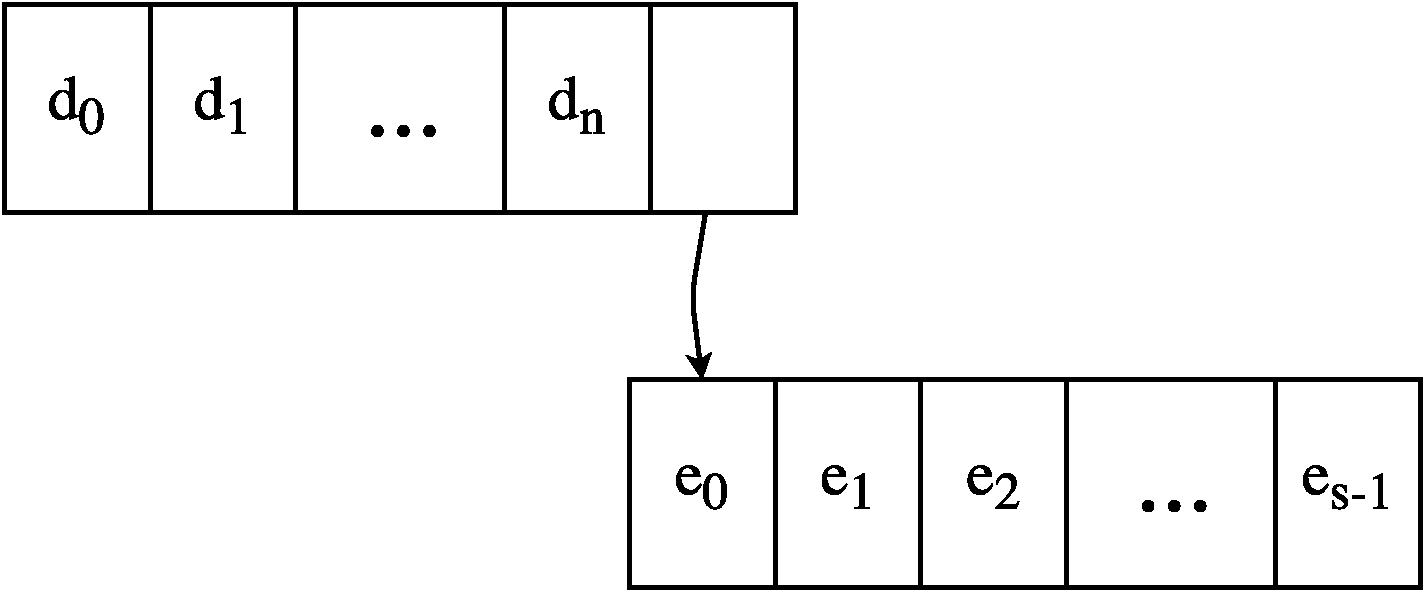
\includegraphics[width=5cm]{diag}
  \end{center}

\end{itemize}
\end{frame}

\defverbatim[colored]\boundproc{
\begin{lstlisting}[language=graciela, style=code, escapechar=\~]
proc p (...)
{pre   ...   pre}
{post  ...  post}
{bound ... bound}
|[ ... p() ... ]|
\end{lstlisting}
}

\defverbatim[colored]\cnfquant{
\begin{lstlisting}[language=graciela, style=code, escapechar=\~]
(% ~\qop~ i : int | 0 < i /\ i < 100 /\ (p(i) \/ q(i)) | ... %)
(% ~\qop~ x : float | x ~\Elem~ xs | ... %)
\end{lstlisting}
}

\defverbatim[colored]\countquant{
\begin{lstlisting}[language=graciela, style=code, escapechar=\~]
(% # i : T | R(i) | P(i) %)
\end{lstlisting}
}

\defverbatim[colored]\constmode{
\begin{lstlisting}[language=graciela, style=code, escapechar=\~]
proc f (const c : int, out r : int) 
    ...
\end{lstlisting}
}

\begin{frame}{Otros cambios}
\begin{itemize}
  \item Los procedimientos y funciones recursivos ahora exigen la definición de una expresión de cota. \boundproc{}

  \item Las cuantificaciones admiten rangos más generales en forma normal conjuntiva. \cnfquant{}
\end{itemize}
\end{frame}

\begin{frame}{Otros cambios}
\begin{itemize}
  \item Se agregó el operador de cuantificación \texttt{count} de Dijkstra\footfullcite{ewd737}. \countquant{}

  \item Se agregó el modo de parámetros Const. \constmode{}

\end{itemize}
\end{frame}

\section{ }

\begin{frame}{Teoría de Conjuntos}
\framesubtitle{Requisito indirecto}
Se hizo necesario proveerlos para facilitar la escritura de aserciones para los Tipos de Dato Abstractos.

\begin{itemize}
  \item{\makebox[2.5cm][l]{Conjuntos      } \ingra|\{ \}| }
  \item{\makebox[2.5cm][l]{Multiconjuntos } \ingra|\{: :\} ó | \Lbag \Rbag}
  \item{\makebox[2.5cm][l]{Secuencias     } \ingra|<< >> ó | \Lseq \Rseq}
  \item{\makebox[2.5cm][l]{Relaciones     } \ingra{rel()} }
  \item{\makebox[2.5cm][l]{Funciones      } \ingra{func()} }
\end{itemize}
\end{frame}

\section{Teoría de Conjuntos}

\subsection*{Algo de código}

\defverbatim[colored]\setops{
\setstretch{1.15}
\begin{lstlisting}[language=graciela, style=code, escapechar=\~]
// Operadores

~\Elem~, elem
~\Notelem~, notelem
!=
==
~\Subsett~, subset
~\Ssubset~, ~\SsubsetAlt~, ssubset
~\Superset~, superset
~\Ssuperset~, ~\SsupersetAlt~, ssuperset
\
~\Intersect~, intersect
~\Union~, union
~\Msum~, msum
#
~\Append~, ++
[]
()
\end{lstlisting}
}

\defverbatim[colored]\setfuncs{
\setstretch{1.15}
\begin{lstlisting}[language=graciela, style=code, escapechar=\~]
// Funciones

toSet()
toMultiset()
rel()
func()
multiplicity()
domain()
codomain()
\end{lstlisting}
}

\begin{frame}{Operadores y funciones}
\begin{columns}
\column[t]{5cm}
\begin{minipage}{0.48\textwidth}
\setops
\end{minipage}
\column[t]{5cm}
\begin{minipage}{0.48\textwidth}
\setfuncs
\end{minipage}
\end{columns}
\end{frame}


\defverbatim[colored]\settheory{
\setstretch{1.4}
\begin{lstlisting}[language=graciela, style=code, escapechar=\~]
var m := ~\Lbag~3, 3, 4, 4, 5~\Rbag~ ~\Msum~ ~\Lbag~5, 5, 7~\Rbag~ : multiset of int;
{ m == ~\Lbag~ 3, 3, 4, 4, 5, 5, 5, 7 ~\Rbag~ }
var i := multiplicity (4, m) : int;
{ i == 2 }
var s := toSet (m) ~\Union~ {~~3~~} : set of int;
{ s == {~~3, 4, 5, 7~~} }
var q := ~\Lseq~'a', 'b', 'c'~\Rseq~ : sequence of char;
var k := q[1] : char;
{ k == 'b' }
var d : function int -> char;
    d := func ({ (i, k), (~~2~~*i, q[0])});
var e : relation int <-> char;
    e := rel  ({ (i, d(i)), (i, q[0]), (i, 'z') });
var a := e (i) ~\Intersect~ {'z'} : set of char;
{ a == { 'z' } }
\end{lstlisting}
}

\begin{frame}{Ejemplos}
\settheory{}
\end{frame}

\subsection*{Implementación}

\begin{frame}{Biblioteca Externa}
\begin{itemize}
  \item Biblioteca externa escrita en C++\footfullcite{cpp-lang}.
  \item Aprovecha la biblioteca estándar \texttt{stdlibc++}.
  \item El manejo de memoria es responsabilidad del compilador.
  \item Se libera el espacio asignado cada vez que salen de alcance.
\end{itemize}
\end{frame}

\section{ }

\begin{frame}{Apuntadores}
\framesubtitle{Recomendación de Araujo y Jiménez}
Esta extensión al lenguaje fue una recomendación explícita de Araujo y Jiménez
por su amplia utilidad para el curso <<Algoritmos y Estructuras II>>. Se permite
declarar variables de tipo apuntador a cualquier otro tipo del lenguaje fuera 
de la teoría de conjuntos.

\begin{itemize}
  \item{\makebox[4.8cm][l]{Declaración           } \ingra|var pt : T~~* | }
  \item{\makebox[4.8cm][l]{Reserva de memoria    } \ingra|new  (pt) | }
  \item{\makebox[4.8cm][l]{Liberación de memoria } \ingra|free (pt) | }
  \item{\makebox[4.8cm][l]{Comparación superficial } \ingra| pt1 == pt2 | }
\end{itemize}
\end{frame}

\section{Apuntadores}

\begin{frame}{Paréntesis}

Asimismo, se extendió el reconocedor sintáctico de los tipos para aceptar el 
uso de paréntesis, a fin de permitir al programador distinguir entre, por 
ejemplo, un arreglo de apuntadores y un apuntador a un arreglo.

\begin{itemize}
  \item{\makebox[4cm][l]{Arreglo de apuntadores } \ingra|var ptarr : array [n] of (T~~*~~) | }
  \item{\makebox[4cm][l]{Apuntador a arreglo    } \ingra|var arrpt : (array [n] of T)* | }
\end{itemize}
\end{frame}

\begin{frame}{Debugging}

Para asegurarnos de que las funciones \texttt{new} y \texttt{free} funcionaban
de la manera esperada, hicimos uso de la herramienta \textit{Valgrind}\footfullcite{valgrind}. 
\begin{itemize}
  \item Toma un ejecutable.
  \item Lo enlaza con sus propias funciones de reserva y liberación de memoria.
  \item Elabora un reporte sobre posibles accesos indebidos y pérdida de memoria 
    dinámica.
\end{itemize}

Gracias a esto, descubrimos varias fugas de memoria y accesos indebidos, específicamente
en el uso de arreglos. La forma en que habíamos implementado inicialmente los arreglos conformantes presentaba fallos y estos fueron solventados exitosamente.
\end{frame}

\subsection*{Aserciones}
\begin{frame}{Lógica de separación}
Para poder expresar aserciones sobre estructuras que hacen uso de apuntadores, 
el Prof. Monascal nos orientó hacia la extensión de la Lógica de Hoare conocida 
como Lógica de Separación\footfullcite{separation-logic}.

\begin{itemize}
  \item No le agrega poder a la Lógica de Hoare.
  \item Agrega expresividad y permite enunciar propiedades complejas de 
  una manera más sucinta.
 \end{itemize}
\end{frame}

\begin{frame}{Lógica de separación, semántica}

\begin{description}
  \item [emp] Es la constante que representa un \textit{heap} vacío. 
  \item [$*$] Es la \textit{conjunción separadora}. $P*Q$ significa que P y Q son verdaderas en porciones disjuntas de la memoria.
  \item [$\mapsto$] Es el operador de \textit{deconstrucción de heap unitario}. $E \mapsto x$ significa que E apunta al fragmento de memoria $x$. Suele usarse de la forma $E \mapsto [l : x, r : y]$, equivalente a $(E \mapsto x) * (E + 1 \mapsto y)$
\end{description}

\end{frame}

\begin{frame}{Lógica de separación, cont.}
\framesubtitle{Ejemplo motivador}

\begin{align*}
  tree(E) \Longleftrightarrow\ &\boldsymbol{if}\ isatom?(E)\ \boldsymbol{then}\ emp \\
             &\boldsymbol{else}\ \exists xy.\ E\mapsto[l: x,\ r: y] * tree(x) * tree(y) \nonumber
\end{align*}

\end{frame}

\begin{frame}{Lógica de separación, cont}
Sin embargo,
\begin{itemize}
  \item Difícil implementación debido a complejas estructuras internas (simulación del heap).
  \item Nuevo sistema formal para estudiantes de cursos introductorios. 
\end{itemize}
\end{frame}

\section*{ }

\begin{frame}{Tipos de Dato Abstractos\footfullcite{dalewalker}\footfullcite{ravelo}}

\begin{itemize}
  \item Recomendación más importante de Araujo y Jiménez.
  \item Centro de la presente extensión al lenguaje Graciela.
  \item Se busca la misma expresividad del lenguaje GCL.
  \item Restricciones y comportamientos verificados a tiempo de ejecución.
\end{itemize}
\end{frame}

\section{Tipos de Dato Abstractos}

\subsection*{Abstracciones}

\begin{frame}{Comportamientos abstractos}
\begin{itemize}
  \item Se definen con la palabra reservada \ingra{abstract}.
  \item Variables internas para establecer propiedades.
  \item Invariante de representación (\ingra{repinv}).
  \item Procedimientos y funciones sin cuerpos, definen una interfaz.
\end{itemize}
\end{frame}

\subsection*{Implementaciones}
\begin{frame}{Implementaciones}
Para aprovechar la definición de un tipo de dato abstracto, es necesario proveer una \textit{implementación} de éste.
\begin{itemize}
  \item Se definen con la palabra reservada \ingra{type}.
  \item Variables internas de \textbf{tipos básicos}, apuntadores, o arreglos.
  \item Invariante de representación (\ingra{repinv}).
\end{itemize}
\end{frame}

\begin{frame}{Implementaciones, cont.}
\begin{itemize}
    \item Se decidió separar el invariante de acoplamiento de la literatura en dos partes
    \begin{itemize}
      \item \textit{relación} de acoplamiento (\ingra{where})
      \item \textit{invariante} de acoplamiento (\ingra{coupinv}).
    \end{itemize}
  \item Por último, una \textit{implementación} también cuenta con procedimientos y funciones. 
  \item Si el TDA especifica un procedimiento o función, \textit{cualquier} \ingra{type} que busque implementarlo debe contar con su propia definición de éste.
\end{itemize}
\end{frame}

\begin{frame}{Tripleta de Hoare}
Si se tiene el procedimiento $\textbf{proc}\ p (Y)$, e $Inv(x)$ es el predicado que condensa todos los
invariantes del valor $x$ si $x$ es de un TDA, entonces se debe cumplir que

\begin{equation*} \label{eqn:tdatriple}
\begin{gathered}
% \frac{
  \{ P[X/Y] \land (\forall x\ |\ x \in X \land isTDA?(x)\ |\ Inv(x) )\}\\
  p\ (X)\\
  \{ Q[X/Y] \land (\forall x\ |\ x \in X \land isTDA?(x)\ |\ Inv(x) )\}
% }{
% }
\end{gathered}
\end{equation*}
\end{frame}

\begin{frame}{Relación \textit{implementa a}}
Por lo tanto, cuando en Graciela se hace una llamada, se genera código para las siguientes aserciones, en orden

\begin{enumerate}
  \item Precondición de la implementación.

  \item Relación e Invariante de acoplamiento.

  \item Invariante de representación de la \textit{implementación}.

  \item Precondición del TDA, si existe.

  \item Invariante de representación del TDA.

  \item \textit{Cuerpo del procedimiento}.


\end{enumerate}
\end{frame}

\begin{frame}{Relación \textit{implementa a}, cont.}
\begin{enumerate}\setcounter{enumi}{6}
  \item Relación e Invariante de acoplamiento.

  \item Invariante de representación del TDA.

  \item Poscondición del TDA, si existe.

  \item Invariante de representación de la \textit{implementación}.

  \item Poscondición de la implementación.
    \begin{itemize}
      \item Si se cumplieron ambas poscondiciones, la ejecución sigue normalmente
      \item Si sólo se cumple la poscondición del la implementación, se emite el
      error <<No se cumple la poscondición>>
      \item Si sólo se cumple la poscondición del TDA, se emite el error <<Este
      procedimiento no implementa el TDA>>
      \item Si ninguna de las dos poscondiciones se cumple, se emiten ambos errores.
    \end{itemize}
\end{enumerate}
\end{frame}

\subsection*{Implementación}

\begin{frame}{Detrás de la escena}
Los invariantes de representación (\ingra{repinv}), y los invariantes  (\ingra{coupinv}) y relaciones de acoplamiento (\ingra{where}) funcionan como rutinas internas que son generadas para cada TDA y cada implementación, y son llamadas en los momentos apropiados. 

Adicionalmente, para cada implementación, se generan rutinas internas para crear, copiar y eliminar objetos de su tipo. 
\end{frame}

\begin{frame}{Modos de parámetros}
Por supuesto, debe ser posible pasar objetos de un TDA en los distintos modos de parámetros del lenguaje Graciela, a saber, In, In-Out, Out y Ref.

\begin{description}
  \item [In]     Se crea en el heap una estructura del tipo apropiado, se copia el parámetro real en ella, pasando un apuntador a esta estructura.
  \item [Out]    Se crea en el heap una estructura del tipo apropiado, vacía, y se pasa un apuntador a esta estructura. Al finalizar el procedimiento, se copia esta estructura sobre el parámetro real.
  \item [In-Out] Combinación de los dos modos anteriores. 
  \item [Ref]    Simplemente se pasa una referencia al parámetro real.
  \item [Const]  Sólo disponible para variables de tipos básicos. 
\end{description}

\end{frame}

\defverbatim[colored]\typevar{
\begin{lstlisting}[language=graciela, style=code, escapechar=\~]
abstract ALista (A)
    ...

type Lista(B) implements ALista(B)
    ...
    proc p (in l : Lista(B))
      ...
\end{lstlisting}
}

\begin{frame}{Variables de tipo}
Una situación bastante frecuente en los TDA es que sus comportamientos son genéricos sobre los tipos que contienen. Por lo tanto, se decidió permitir
especificar los TDAs y sus implementaciones con variables de tipo. 

\typevar

En Graciela, estas variables de tipo siempre serán instanciadas en tipos básicos, y los procedimientos definidos dentro de \ingra{ALista(A)} y \ingra{Lista(B)} no pueden hacer suposiciones sobre \ingra{A} o \ingra{B} más allá de que son comparables, mostrables y legibles por teclado. 
\end{frame}

\defverbatim[colored]\typevarr{
\begin{lstlisting}[language=graciela, style=code, escapechar=\~]
var miListaInt  : Lista (int);
var miListaChar : Lista (char);

p(miListaInt);
p(miListaChar);
\end{lstlisting}
}

\begin{frame}{Variables de tipo, cont.}
Si se crea una variable de un TDA dentro del programa principal, o dentro de un procedimiento en el alcance global, se deben especificar tipos básicos para
cada una de las variables de tipo dadas en la declaración \ingra{type}.

\typevarr

A tiempo de compilación, se generan dos tipos de estructura, y para cada una, 
una copia de cada procedimiento, función, y rutina interna, cambiando únicamente
el tipo que sustituye a la variable de tipo \ingra{B}. Esto podría parecer 
exagerado, pero de hecho es la misma técnica de plantillas que utiliza el 
compilador de C++.
\end{frame}

\defverbatim[colored]\typevarrr{
\begin{lstlisting}[language=graciela, style=code, escapechar=\~]
type Lista(B) implements ALista(B)
    ...
    proc q (in l : Lista(B), in b : B)
      ...

var miListaInt  : Lista (int);
var miListaChar : Lista (char);

q (miListaInt,   3 )
q (miListaChar, '3')
\end{lstlisting}
}

\begin{frame}{Variables de tipo, cont.}
Por último, la verificación de tipos para llamadas a procedimientos de TDAs 
es capaz de reconocer el tipo apropiado para el segundo parámetro de un procedimiento como

\typevarrr
\end{frame}

\section{Extras}

\defverbatim[colored]\pragma{
\begin{lstlisting}[language=graciela, style=code, escapechar=\~]
/*% LANGUAGE Trace %*/
\end{lstlisting}
}

\begin{frame}{Apoyo al programador}
\begin{itemize}
  \item Se simplificó el proceso de compilación, ahora basta con usar el comando \texttt{graciela}. Adicionalmente, se provee el comando \texttt{rungraciela}, que compila y ejecuta un programa en un solo paso.
  \item Se desarrollaron resaltadores sintácticos de Graciela para los editores Vim y Sublime Text. Adicionalmente, para este último editor se escribieron plantillas (\textit{Snippets}) de código.
  \item Por otro lado, se agregó al lenguaje la capacidad de imprimir trazas dentro de funciones con el pragma
  \pragma
  que habilita la familia de funciones \ingra{trace()}.
\end{itemize}
\end{frame}


\section{ }

\section{Resultados}
\begin{frame}{Resultados}
\begin{itemize}
  % \item Cambios en la gramática. Bloque principal, poscondición y aserciones.
  \item Verificaciones para arreglos. Arreglos multidimensionales.
  \item Cotas en subrutinas
  \item Cuantificaciones más flexibles.
  \item Manejo manual de apuntadores.
  \item Teoría de conjuntos.
  \item Tipos de Dato Abstractos e Implementaciones.
  \item Apoyo al programador.
\end{itemize}
\end{frame}

\section{Conclusiones}
\begin{frame}{Conclusiones}
\begin{itemize}
  \item Para el \textit{Front-End} se utilizó la biblioteca de análisis sintáctico \textit{Megaparsec}\footfullcite{megaparsec}.
  \item Para el \textit{Back-End}
  se aprovechó la familia de software LLVM, a través de las bibliotecas \textit{llvm-general}\footfullcite{llvm-general} y \textit{llvm-general-pure}\footfullcite{llvm-general-pure}.
  \item El producto final de este proyecto es un lenguaje, junto con su compilador, diseñado para la enseñanza de los cursos de Algoritmos y Estructuras I y II de la USB.
\end{itemize}
\end{frame}

\section{Recomendaciones}
\begin{frame}{Recomendaciones}
\begin{itemize}
  % \item Compilación de varios archivos.
  % \item Tipos enumerados.
  \item Tipos Algebráicos Libres.
  % \item Escribir la biblioteca externa en Graciela, en lugar de en C++.
  % \item Colecciones de colecciones.
  \item Variables de tipo instanciadas en tipos no-básicos.
  % \item Subrutinas correcursivas (tupla de cotas).
  \item Lógica de separación.
\end{itemize}
\end{frame}

\begin{frame}[c]{\empty}
\begin{center}
\Huge{¿Preguntas?}
\end{center}
\end{frame}

\end{document}
